\chapter{Realizace}

V této kapitole je popsáno, jak byly poznatky z kapitol předešlých zapojeny do hry \verb|trogASR|. Nalezneme zde především ukázky a příklady.

Pro popis zacházení s jednotlivými částmi aplikace slouží příloha \ref{appendix:user_doc}.

\section{Nasazení}

V současnosti lze aplikaci \verb|trogASR| nalézt na \url{http://trogasr-trogasr.rhcloud.com/}. Toto nasazení je pouze demonstrační. V dohledné době proběhne nasazení finální verze na některý z aplikačních serverů \nom{ÚFAL}{Ústav Formální a Aplikované Lingvistiky}.

Zatím na zmíněném hostingu běží hra v {\sl DEBUG} módu. Hosting samotný má své problémy --- bylo využito pouze verze zdarma --- proto se může stát, že aplikace bude místy krátkodobě nedostupná.

Pečlivě dokumentovaný zdrojový kód aplikace zájemce nalezne na \url{https://github.com/Heehaaw/trogASR}.

\section{Zobrazení}

\begin{figure}[h]
	\centering
	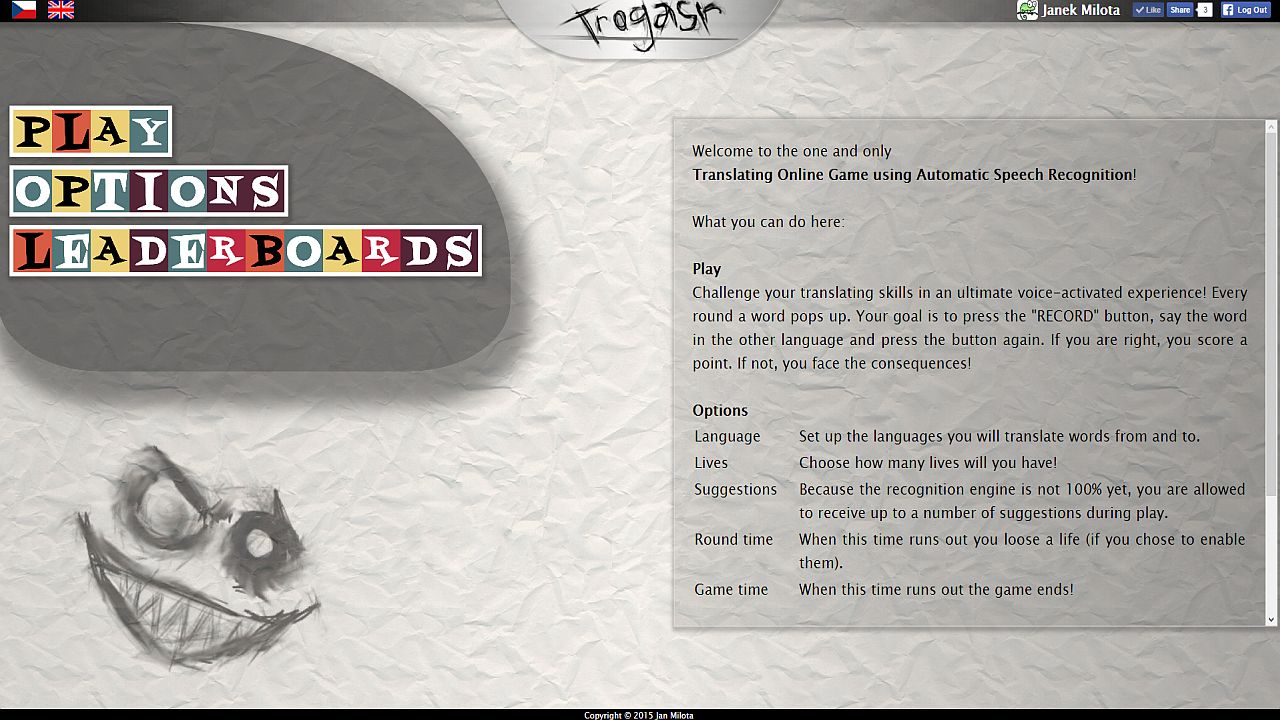
\includegraphics[width=140mm,height=80mm]{img/title_screen.jpg}
	\caption{Ukázka úvodní obrazovky.}
	\label{fig:title}
\end{figure}

Obrázek \ref{fig:title} ukazuje, jak vypadá úvodní obrazovka aplikace. Tato slouží jako základní rozcestník aplikace, nalezneme zde jednoduchou uživatelskou příručku a veškeré nastavovací a ovládací prvky.

\begin{figure}[h]
	\centering
	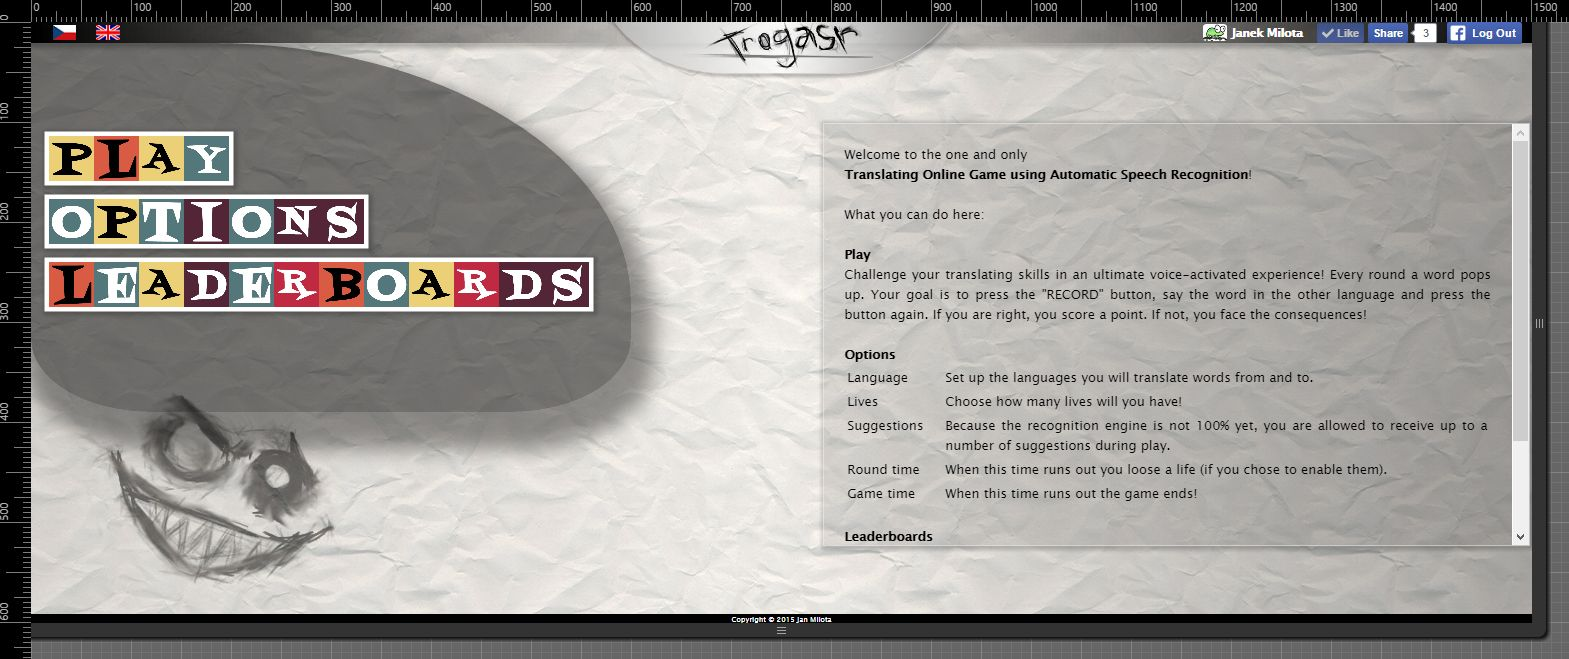
\includegraphics[width=140mm,height=50mm]{img/title_stretch.jpg}
	\caption{Ukázka úvodní obrazovky v nestandardním rozlišení.}
	\label{fig:title_stretch}
\end{figure}

Obrázek \ref{fig:title_stretch} ukazuje zobrazení aplikace ve velmi nestandardním rozlišení. Můžeme vidět, že i přes obskurnost zobrazovacího média se aplikace chová velmi dynamicky a vypadá pořád přiměřeně efektně.

Všechny grafické prvky jsou navrženy s ohledem na možnost zobrazení na inferiorním zobrazovacím zařízení, jsou tedy pro počítačové monitory zdánlivě příliš velké. V menších rozlišeních a na menších displejích však tato velikost výrazně ulehčuje uživatelskou interakci.

\section{Kompetitivita}

Hra \verb|trogASR| má být hnána touhou překonat své přátele a nahrát víc bodů. Proto na spodní části obrázku \ref{fig:competitivity} můžeme vidět, jak vypadá zobrazení žebříčků, kde se fakta o bodech hráčů zaznamenávají. 

Aby byl kompetitivní aspekt hry fér, nemohou být žebříčky hromadné pro všechna nastavení hry. Proto každá kombinace možností nastavení má žebříčky své vlastní. Nastavení pro žebříčky na obrázku \ref{fig:competitivity} ukazuje jeho horní polovina.

\begin{figure}[h]
	\centering
	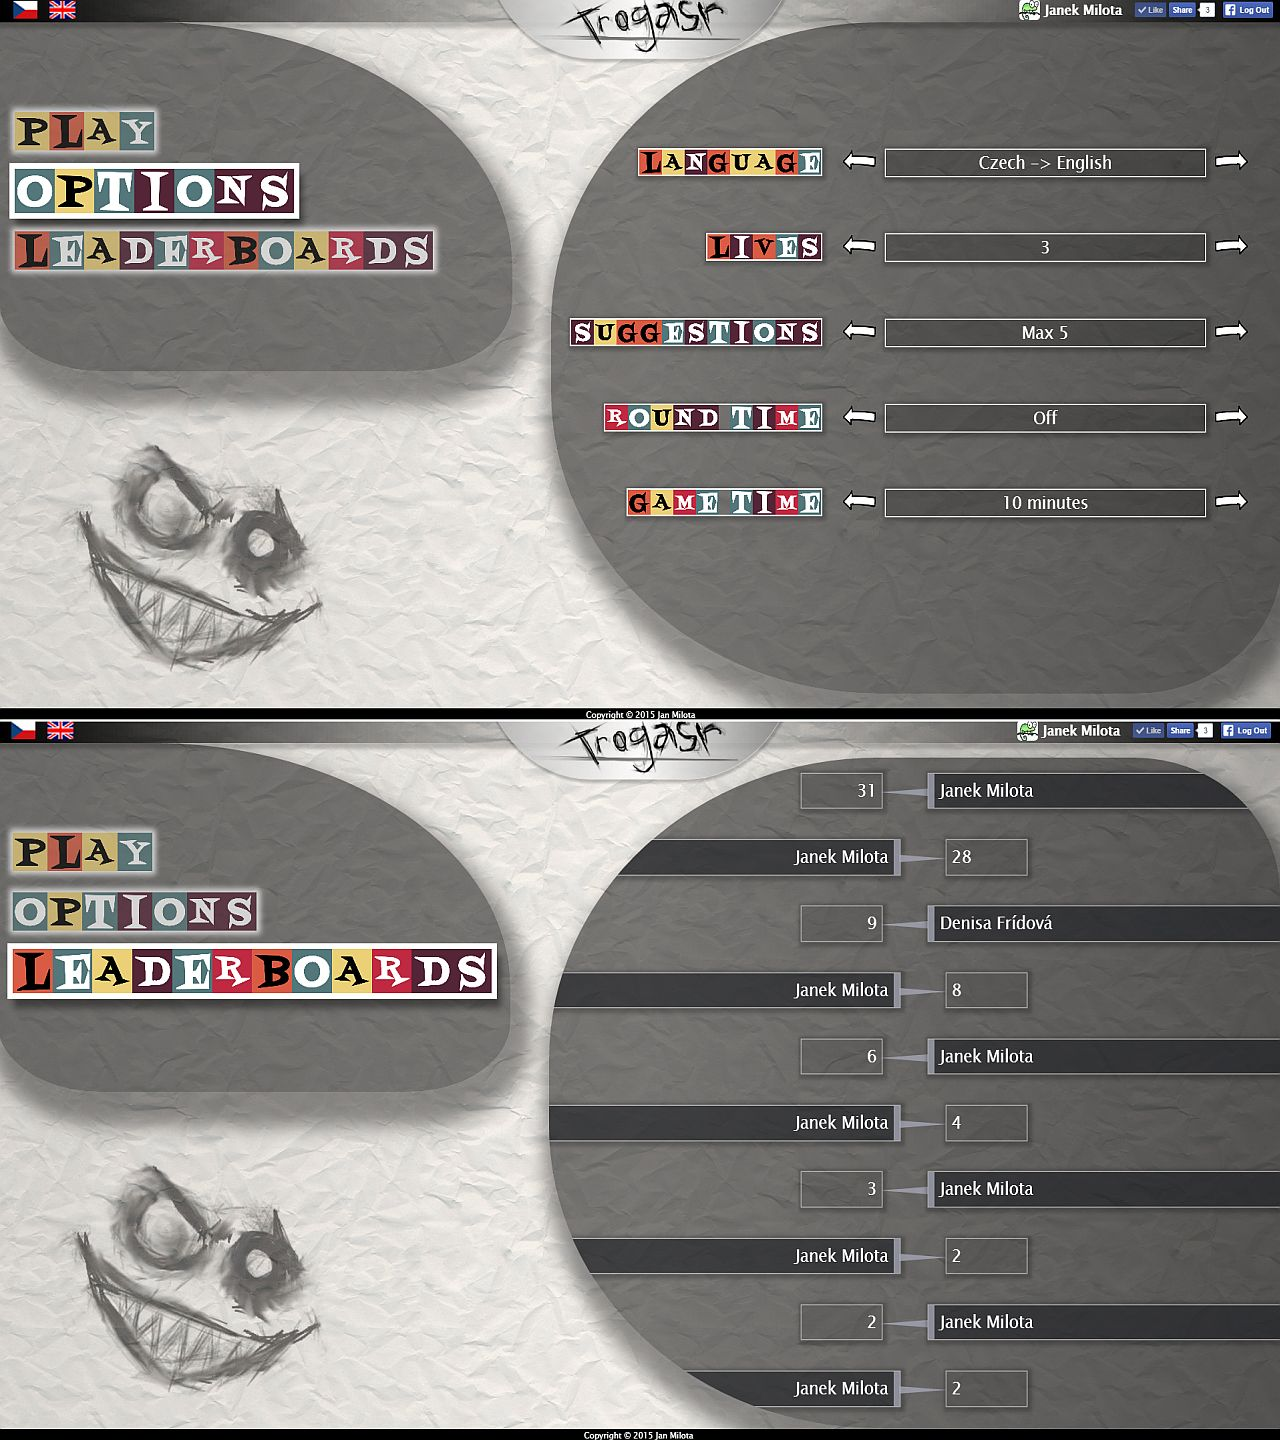
\includegraphics[width=140mm,height=140mm]{img/competitivity.jpg}
	\caption{Obrazovky nastavení a žebříčků.}
	\label{fig:competitivity}
\end{figure}

\section{Výuka hrou a crowdsourcing}

Hra \verb|trogASR| má ve výsledku tři hlavní účely: bavit hráče, zdokonalovat jeho jazykové schopnosti a získávat data pro platformu \verb|CloudASR|. Všechny tyto procesy jsou realizovány veskrze nenásilnou formou. Na obrázku \ref{fig:game} je možno spatřit, jak vypadá obrazovka herní. 

Na obrázku \ref{fig:game} lze také zahlédnout co se stane, není-li vyřčené slovo rozpoznáno. V daném příkladu rozpoznávač nevrátil nic, nebo pouze prázdné řetězce. Hráč v tomto případě měl zapnuté nastavení nápověd, proto se mu zobrazil panel s nápovědami obsahující pouze jedu --- správnou --- volbu.

V případě, že rozpoznávač hlasu vrátí nějaký výstup, je tento zobrazen přesně ve formě, v jaké byl získán. Stává se tedy, že hráč má snadnou volbu správného výběru, protože pouze jedno slovo z nabízených dává smysl.

I touto formou ale hráč dostává informace o překladu slova. Nemusí nutně slovo říci správně a přesně, stačí, když následně dokáže vybrat správný překlad z nabízených možností. Tento fakt zjednodušuje proces předání výukového materiálu hráči a zároveň zpříjemňuje hráči jeho prožitek.

Zároveň po celou dobu herního sezení, kdy je hráč zabaven hrou, motivován umístěním v žebříčcích a vzděláván v překladu slov a frází, zapojuje se rád a dobrovolně do procesu crowdsourcingu.

\begin{figure}[h]
	\centering
	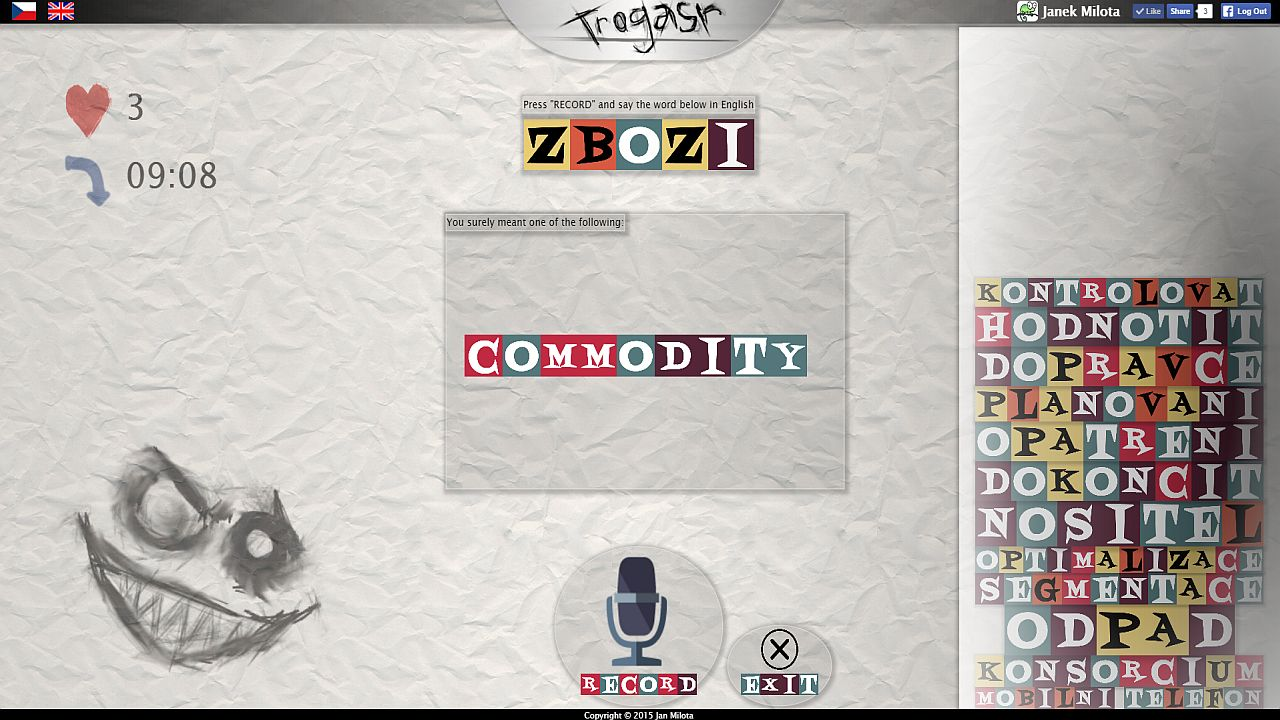
\includegraphics[width=140mm,height=80mm]{img/game.jpg}
	\caption{Herní obrazovka.}
	\label{fig:game}
\end{figure}

\section{Uživatelské ohlasy}

Aplikaci \verb|trogASR| do dnešního dne příliš mnoho uživatelů nestřetlo. Spatřila světlo světa poněkud nedávno a vystavena je pouze chvíli. Ti uživatelé, kteří se však do styku se hrou dostali, podávají z velké části pozitivní zpětnou vazbu.

Součástí většiny pozitivní zpětné vazby je zmínka o pěkném grafickém provedení a o intuitivnosti nastavení a ovládání hry.

Hlavním negativem uživatelské odezvy je fakt, že samotné rozpoznávání řeči jen málokdy vrátí relevantní textové řetězce. Není se však čemu divit. Samotné rozpoznávání řeči je o to kvalitnější, čím větší má nasbíranou datovou základnu. Hra \verb|trogASR| má sloužit právě k obohacování této základny.